% Corps du matériel supplémentaire, partagé par sc_reborn_supplementaire.tex
% (fichier séparé pour la soumission) et sc_reborn_ijpe.tex (annexé à la fin de l'article).

\section*{S0. Vue détaillée de la démarche}

La figure~\ref{fig:S1} détaille la démarche résumée à la figure 1 de l'article. Pour chacun des trois blocs, elle précise les données d'entrée, les traitements et les sorties : la génération des crises étiquetées et de leurs quatre versions (simuler), l'ajustement de la courbe de résilience et le calcul des indicateurs (mesurer), puis l'apprentissage du réseau bayésien causal et ses trois usages (apprendre). Des vignettes illustrent une trajectoire, une courbe ajustée et la structure du réseau appris.

\begin{center}\begin{minipage}{\textwidth}\centering
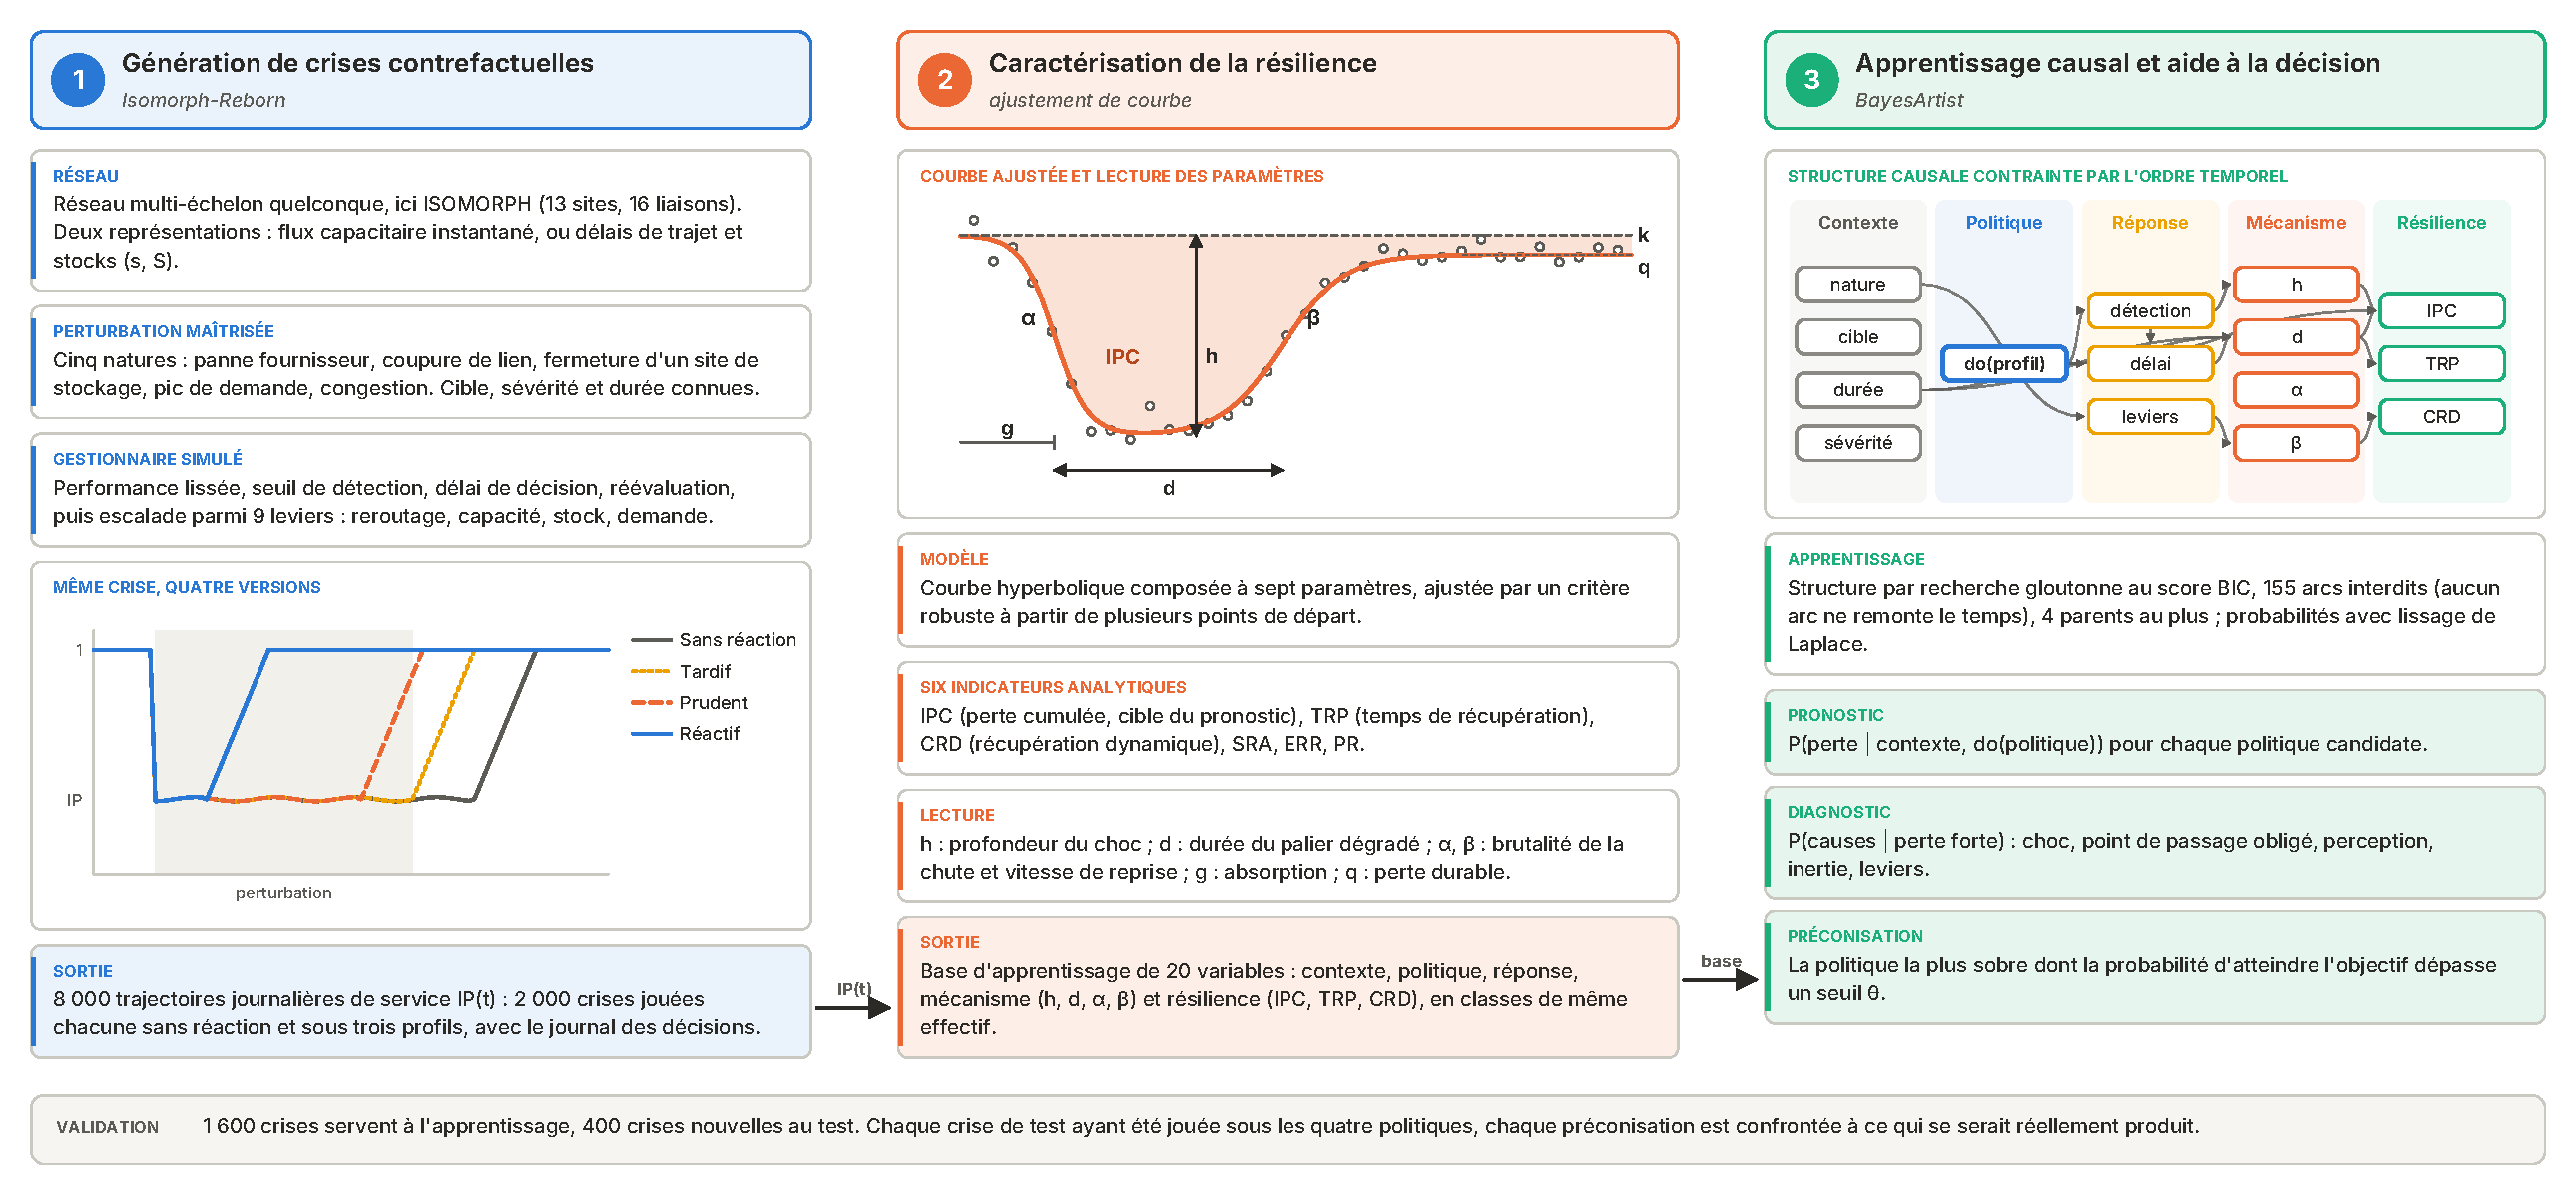
\includegraphics[width=\textwidth]{figures/Fig1_demarche.pdf}
\captionof{figure}{Démarche détaillée en trois blocs : entrées, traitements et sorties de chaque bloc.}\label{fig:S1}
\end{minipage}\end{center}

\section*{S1. Compléments sur le générateur de scénarios (Simuler)}

Cette partie reprend les détails de modélisation retirés de la section 3 de l'article pour respecter la longueur demandée par la revue.

\subsection*{Positionnement par rapport à ISOMORPH}

Le tableau~\ref{tab:S1} résume les écarts entre la démarche proposée et le jumeau numérique ISOMORPH.

\begin{center}\begin{minipage}{\textwidth}
\captionof{table}{Positionnement de la démarche par rapport à ISOMORPH.}
\label{tab:S1}
\footnotesize
\begin{tabularx}{\textwidth}{@{}LLL@{}}
\toprule
\textbf{Dimension} & \textbf{ISOMORPH} & \textbf{Démarche proposée} \\
\midrule
Réseau & 13 nœuds, destination unique, pas journalier & Réseau multi-échelon quelconque ; réseau paramétrique à redondance partielle et réseau ISOMORPH d'origine comme références \\
Dynamique & Stocks gérés en (s, S) & Deux représentations emboîtées : flux capacitaire instantané, ou délais de trajet et de production avec stocks (s, S) à couverture réglable \\
Perturbations & Aléatoires, non étiquetées & Cinq natures maîtrisées : cible, date, durée et sévérité connues \\
Décisions & Paramètres fixés avant la simulation & Gestionnaire simulé réagissant en cours de crise \\
Expérimentation & Tirages indépendants & Même crise rejouée sous plusieurs comportements de gestion \\
\bottomrule
\end{tabularx}
\end{minipage}\end{center}

\subsection*{Réseaux de référence}

Deux réseaux servent de référence (tableau~\ref{tab:S2}). Le réseau paramétrique comporte trois échelons : trois usines, neuf entrepôts et un client final. Chaque entrepôt est approvisionné par une usine principale, par une usine de secours via un lien de moindre capacité et, pour un entrepôt sur trois, par une troisième usine. La redondance est donc partielle par construction : la perte de la voie principale d'un entrepôt ne peut être que partiellement compensée par ses voies de repli, comme dans la plupart des réseaux réels où la double source reste coûteuse.

Le réseau ISOMORPH reprend la topologie d'origine (Fig.~3 de l'article) : treize villes reliées par seize liaisons, avec un hub et cinq échelons intermédiaires entre les sources et le client. Le fichier d'origine ne fixant pas toutes les grandeurs nécessaires, trois hypothèses complètent sa description. La capacité de chaque liaison est tirée à plus ou moins 10 \% autour de sa valeur d'origine. La capacité de production de chaque source est fixée à 0,8 fois la capacité cumulée de ses liaisons sortantes : à 1,0, la production ne pourrait jamais constituer un goulot et le report de charge vers les sites de production sains serait sans effet. Le dernier kilomètre est enfin supposé illimité ; les deux derniers sites de stockage avant le client n'ont alors ni capacité propre ni liaison sortante limitée, et échappent aux leviers d'expédition.

Les valeurs nominales des deux réseaux figurent au tableau~\ref{tab:S2}.

\begin{center}\begin{minipage}{\textwidth}
\captionof{table}{Caractéristiques des deux réseaux de référence (valeurs nominales).}
\label{tab:S2}
\footnotesize
\begin{tabularx}{\textwidth}{@{}LLL@{}}
\toprule
\textbf{Élément} & \textbf{Réseau paramétrique} & \textbf{Réseau ISOMORPH} \\
\midrule
Sites et échelons & 3 usines, 9 entrepôts, 1 client & 13 villes, 16 liaisons, 1 hub, 5 échelons intermédiaires \\
Capacité de production d'une source (unités par jour) & 200 à 320 & 0,8 fois la capacité de ses liaisons sortantes \\
Capacité des liaisons (unités par jour) & Voie principale 60 à 110 ; voie de secours 15 à 35 ; troisième voie 10 à 20 & Valeur d'origine $\pm$ 10 \% ; dernier kilomètre illimité \\
Capacité d'expédition d'un site de stockage (unités par jour) & 50 à 100 & Portée par les liaisons sortantes \\
Délai de trajet, représentation temporelle (jours) & 0 par défaut, réglable & 1 à 8 (valeurs d'origine) \\
Délai de production, représentation temporelle (jours) & 0 par défaut, réglable & 0 par défaut, réglable \\
Part des articles critiques dans la demande & 15 \% à 45 \% & 15 \% à 45 \% \\
Fluctuation journalière de la demande & $\pm$ 3 \% à $\pm$ 8 \% & $\pm$ 3 \% à $\pm$ 8 \% \\
\bottomrule
\end{tabularx}
\end{minipage}\end{center}

\subsection*{Règles de la représentation temporelle}

Trois règles complètent la représentation. Chaque jour, un site de stockage sert d'abord les besoins du jour, puis le recomplètement des sites en aval, et la répartition privilégie la liaison principale avant les liaisons de secours. Les articles critiques et ordinaires sont agrégés dans les stocks, la priorité aux articles critiques ne s'appliquant qu'au service du client. Enfin, les liaisons vers le client sont servies le jour même : avec un délai sur ces liaisons, le client recevrait aujourd'hui ce qu'il a commandé la veille, et l'indicateur baisserait à chaque hausse de la demande d'un jour à l'autre, même sans perturbation ; il mesurerait alors le bruit de la demande et non la disponibilité du réseau.

Avant toute observation, le réseau est simulé sans perturbation pendant une pré-chauffe de 60 jours, qui amène les stocks et la matière en route à leur régime établi. Cette pré-chauffe est commune aux quatre versions d'une même crise (section 3.6 de l'article).

Les deux représentations sont emboîtées. À délais nuls, la représentation temporelle reproduit presque exactement la représentation par flux : l'écart moyen de l'indicateur de performance reste compris entre 0,00025 et 0,002 selon les cas testés. Avec des délais, en revanche, les stocks modifient profondément la réponse du réseau aux chocs, dans une mesure qui dépend de la couverture et de la nature du choc ; la section 6.5 de l'article en analyse la sensibilité.

\subsection*{Calibration de la demande de référence}

Dans la représentation par flux, le volume livrable $F(t)$ d'un jour est la quantité maximale que le réseau peut acheminer des sources au client compte tenu de toutes ses capacités, dégradées ou renforcées ce jour-là. Cette formulation fait apparaître naturellement les goulots d'étranglement : c'est souvent la capacité d'expédition des sites de stockage, et non la production, qui limite le service. Dans la représentation temporelle, $F(t)$ désigne le volume que la circulation de la matière et les stocks permettent effectivement de livrer ce jour-là (section 3.3 de l'article). Dans les deux cas, ce volume sert en priorité les articles critiques, et la performance du jour est mesurée par un taux de service pondéré, dans lequel les articles critiques comptent triple :

Dans la représentation temporelle, $F_{\mathrm{inc}}$ et $F_{\mathrm{nom}}$ sont les volumes que la circulation de la matière permet effectivement d'écouler, au plus égaux au volume maximal de la représentation par flux. Le second terme ne suffit plus à garantir l'absence de dégradation : les recomplètements par à-coups et les délais peuvent laisser une demande non servie un jour donné, même sans perturbation. La demande de référence est donc vérifiée par simulation. Chaque scénario est simulé sans perturbation, pré-chauffe comprise, avec sa propre série de fluctuations, et $D_{0}$ est la plus grande demande entière au plus égale à $D_{\mathrm{max}}$ qui est servie intégralement chaque jour :

$\mathrm{IP}_{d}(t)$ désigne l'indicateur de performance obtenu sous une demande de référence $d$, les niveaux s et S étant recalculés par l'équation~(2) de l'article pour chaque demande essayée. La recherche procède par dichotomie sur les entiers et ne fait qu'abaisser $D_{\mathrm{max}}$ ; la valeur retenue est toujours vérifiée par simulation. Lorsque même une demande d'une unité n'est pas servie intégralement, la couverture de stock est trop faible au regard des fluctuations et des délais : le scénario n'admet aucun régime nominal sans dégradation, et le plan d'expériences est refusé plutôt que poursuivi avec une demande arbitraire. Cette condition de faisabilité relie directement la couverture de stock, les délais d'approvisionnement et la variabilité de la demande.

\subsection*{Leviers de stock en représentation temporelle}

Dans la représentation temporelle, les deux leviers de stock changent de mécanisme. Le pré-positionnement (D7) relève temporairement les niveaux s et S des sites de stockage et déclenche une commande immédiate. Le déstockage (D6) libère une réserve de sécurité tenue à l'écart du stock ordinaire : elle n'est pas visible de la politique de commande et ne sert que la demande que le stock ordinaire n'a pu satisfaire.

Ce choix n'est pas anodin. Injectée directement dans le stock ordinaire, la même quantité faisait passer certains sites au-dessus de leur point de commande. Ils sautaient alors un recomplètement, le besoin manquant remontait jusqu'aux sources, qui restaient à l'arrêt un jour de panne, et la capacité de production ainsi perdue ne se rattrapait pas : sur un cas mesuré, le levier réduisait le volume livré au lieu de l'accroître. Une intervention d'urgence sur les stocks peut donc perturber le signal de réapprovisionnement qu'elle devait soulager. La réserve séparée garantit que le déstockage ne réduit jamais le volume livré. Les deux leviers de stock excluent enfin les sites de stockage sans capacité propre et à liaisons sortantes illimitées, sur lesquels ils n'ont pas de prise (section 3.2 de l'article).

\subsection*{Niveau de tension et contenu des observations}

Toutes les valeurs posées par hypothèse faute de données de terrain peuvent être modifiées : capacités, effets des leviers, caractéristiques des profils, hypothèses qui complètent le réseau ISOMORPH et paramètres de la représentation temporelle. Pour explorer des contextes contrastés, un niveau de tension global, de 0 à 100, déplace simultanément quatre groupes d'hypothèses : l'intensité et la durée des chocs, la tension du réseau, l'efficacité des leviers et la réactivité des gestionnaires. Le niveau 50 correspond aux valeurs nominales présentées ici. Le niveau 0 décrit un réseau surcapacitaire soumis à des chocs brefs et géré par des décideurs très réactifs ; le niveau 100 décrit des chocs de 12 à 32 jours sur un réseau saturé, avec des leviers peu efficaces et des délais de décision allant jusqu'à 12 jours. Lorsque le réseau est imposé, ce niveau continue de piloter la sévérité et la durée des chocs, la tension entre demande et capacité, l'efficacité des leviers et la réactivité des gestionnaires, mais ne modifie pas les capacités du réseau, qui viennent de sa description. Il ne touche pas non plus aux délais ni à la couverture de stock, qui relèvent de la représentation du réseau et non de l'intensité de la crise.

Chaque version d'une crise constitue une observation complète, qui réunit le contexte du réseau (identité et taille du réseau, demande de référence, part des articles critiques), la perturbation subie, le journal des décisions (date de détection, leviers mobilisés et dates d'engagement) et la trajectoire journalière de performance. Les niveaux de stock et la matière en route ne sont pas enregistrés : la base décrit une crise par ses causes, ses décisions et le service rendu, et non par l'état interne du réseau. Des grandeurs descriptives simples, performance minimale, performance cumulée perdue et délai de retour à la normale, servent au contrôle de la base. La caractérisation de la résilience proprement dite est confiée au bloc 2.

\section*{S2. Signatures des dysfonctionnements sur la courbe de résilience}

Les paramètres de la courbe relient la trajectoire observée aux mécanismes décrits en section 3 de l'article. Le tableau~\ref{tab:S3} résume les signatures attendues ; il constitue un ensemble d'hypothèses que l'analyse des résultats et l'apprentissage causal permettent de confirmer ou de nuancer.

\begin{center}\begin{minipage}{\textwidth}
\captionof{table}{Signatures des dysfonctionnements sur la courbe de résilience.}
\label{tab:S3}
\footnotesize
\begin{tabularx}{\textwidth}{@{}LLL@{}}
\toprule
\textbf{Phénomène} & \textbf{Signature attendue sur la courbe} & \textbf{Origine probable} \\
\midrule
Absorption du choc & $h$ faible, $g$ élevé & Marges de capacité, voies de secours suffisantes \\
Absorption par les stocks & $h$ faible ou nul, $g$ élevé & Couverture de stock élevée au regard de la durée du choc \\
Rupture brutale & $h$ élevé, $\alpha$ élevé & Coupure ou fermeture sévère, réseau sous tension \\
Rupture différée & $g$ élevé, puis $h$ élevé & Stocks épuisés en cours de crise, matière en route insuffisante \\
Dégradation progressive & $\alpha$ faible & Congestion diffuse, pic de demande modéré \\
Crise prolongée & $d$ élevé & Perturbation longue, détection tardive, inertie décisionnelle \\
Reprise retardée & $d$ supérieur à la durée du choc & Reconstitution des stocks et de la matière en route après le retour des capacités \\
Reprise rapide & $\beta$ élevé, TRP faible & Levier efficace engagé tôt \\
Perte durable & $q$ $<$ 0 & Capacité non restaurée à la fin de la période, stock épuisé \\
Sur-récupération & $q$ $>$ 0 & Leviers maintenus après la fin de la perturbation \\
\bottomrule
\end{tabularx}
\end{minipage}\end{center}

\section*{S3. Sensibilité à la couverture de stock : valeurs détaillées}

Le tableau~\ref{tab:S4} donne les valeurs représentées à la figure 10 de l'article.

\begin{center}\begin{minipage}{\textwidth}
\captionof{table}{Crises produisant une baisse de service visible, sur 60, selon la couverture de stock (réseau ISOMORPH, sans réaction).}
\label{tab:S4}
\footnotesize
\begin{tabularx}{\textwidth}{@{}LLLLLLLL@{}}
\toprule
\textbf{Nature} & \textbf{Flux} & \textbf{3 / 10 j} & \textbf{2 / 5 j} & \textbf{1 / 3 j} & \textbf{0,5 / 1,5 j} & \textbf{0,25 / 0,75 j} & \textbf{0,1 / 0,3 j} \\
\midrule
Panne fournisseur & 34 & 0 & 0 & 0 & 0 & 0 & 9 \\
Coupure de lien & 36 & 11 & 21 & 27 & 33 & 38 & 43 \\
Fermeture d'un site de stockage & 34 & 14 & 23 & 36 & 43 & 47 & 39 \\
Pic de demande & 38 & 57 & 60 & 60 & 60 & 60 & 60 \\
Congestion & 38 & 27 & 39 & 55 & 59 & 60 & 59 \\
\bottomrule
\end{tabularx}
\end{minipage}\end{center}
